\documentclass{llncs}
\pagestyle{plain}
\usepackage[show]{ed}
\usepackage[utf8]{inputenc}
\usepackage{paralist}
\usepackage{xspace}
\usepackage{amsfonts,amstext}
\usepackage{listings}
\lstset{columns=fullflexible,basicstyle=\sf}
\usepackage{wrapfig}
\usepackage[style=alphabetic,backend=bibtex,isbn=false]{biblatex}
\usepackage{tikzinput}
\usetikzlibrary{backgrounds,shadows,shapes,fit,arrows,mmt,backgrounds,positioning}
\usetikzlibrary{decorations.pathmorphing}

\addbibresource{../../lib/kbibs/kwarcpubs.bib}
\addbibresource{../../lib/kbibs/extpubs.bib}
\addbibresource{../../lib/kbibs/kwarccrossrefs.bib}
\addbibresource{../../lib/kbibs/extcrossrefs.bib}
\addbibresource{rest.bib}% add bibs here!
\renewbibmacro*{event+venue+date}{}
\renewbibmacro*{doi+eprint+url}{%
  \iftoggle{bbx:doi}
    {\printfield{doi}\iffieldundef{doi}{}{\clearfield{url}}}
    {}%
  \newunit\newblock
  \iftoggle{bbx:eprint}
    {\usebibmacro{eprint}}
    {}%
  \newunit\newblock
  \iftoggle{bbx:url}
    {\usebibmacro{url+urldate}}
    {}}
  
\usepackage{hyperref}
\title{REGULAR-T1: Knowledge-Based Interoperability for Mathematical Software Systems}
\author{
Michael Kohlhase\inst{1} 
Dennis M\"uller\inst{1} 
Markus Pfeiffer\inst{3} 
Florian Rabe\inst{2} 
Nicolas~M.~Thiéry\inst{4} 
Victor Vasilyev\inst{3} 
Tom Wiesing\inst{1}
}

\institute{
   FAU Erlangen-N\"urnberg
   \and Jacobs University Bremen
   \and University of St~Andrews 
   \and Universit\'e Paris-Sud
}
\begin{document}
\maketitle
\begin{abstract}
  There is a large, open-source ecosystem of mathematical software systems that collect and
  classify, compute with, prove statements about, and visualize mathematical objects and
  models. Individually, these systems are optimized for particular domains and
  functionalities and together they cover many, but no system covers all needs of
  practical and theoretical mathematics. System integrations exist, but are ad-hoc and
  have scalability and maintainability issues. In particular, there is not yet an
  interoperability layer that combines them into a virtual research environment (VRE) for
  mathematics.
  
  The OpenDreamKit project, which aims at a mathematical VRE toolkit, proposes the
  Math-in-the-Middle (MitM) paradigm, an interoperability framework based on a flexiformal
  representation of mathematical knowledge and aligns this with system-generated interface
  theories. In this paper we instantiate the MitM paradigm with a concrete domain
  development and evaluate it on a distributed computing case study involving GAP,
  SageMath and Singular.
\end{abstract}
\newpage
\setcounter{tocdepth}{3}
\newpage
\tableofcontents
\section{Introduction}\label{sec:intro}

\begin{newpart}{MK: adapted from Tom's Thesis}
There is a large and vibrant ecosystem of open-source mathematical software systems.
These systems can range from calculators, which are only capable of performing simple
computations, via mathematical databases (curating collections of a mathematical objects)
to powerful modeling tools and computer algebra systems (CAS). 

Most of these systems are very specific -- they focus on one or very few aspects of
mathematics.  For example, the ``Online Encyclopedia of Integer Sequences''
(OEIS~\cite{Sloane:oeis12,oeis}) focuses on sequences over $\mathbb{Z}$ an their
properties and the ``L-Functions and Modular Forms Database''
(LMFDB)~\cite{Cremona:LMFDB16,lmfdb:on} objects in number theory pertaining to Langland's
program.  GAP~\cite{GAP:on} excels at discrete algebra, whereas
SageMath~\cite{SageMath:on} focuses on Algebra and Geometry in general, and
Singular~\cite{singular:on} on polynomial computations, with special emphasis on
commutative and non-commutative algebra, algebraic geometry, and singularity theory.

For a mathematician however (a user; let us call her Jane) the systems themselves are not relevant, instead she only cares about being able to solve problems. 
Typically, it is not possible to solve a mathematical problem using only a single program. 
Thus Jane needs to work with multiple systems and combine the results to reach a solution. 
Currently there is very little help with this practice, so Jane has to isolate sub-problems the respective systems are amenable to, formulate them into the respective input language, collect results, and reformulate them for the next system a tedious and error-prone process at best, a significant impediment to scientific progress in its overall effect. 
Solutions for some situations certainly exist, which can help get Jane unstuck, but these are ad-hoc and for specific, often-used system combinations only. 
Each of these requires a lot of maintenance and does not scale to a larger set of specialist systems. 

The OpenDreamKit project, which aims at a mathematical VRE toolkit, proposes the Math-in-the-Middle (MitM~\cite{DehKohKon:iop16}) Paradigm, an interoperability framework based on a flexiformal
representation of mathematical knowledge and aligns this with system-generated interface
theories. 

In this paper we instantiate the MitM paradigm with a concrete domain development and
evaluate it on a distributed computing GAP, SageMath and Singular.\ednote{ we generally we
  want to show that the promises in the CICM paper become reality.}

We will use the following example as a running example: Jane wants to act on singular
polynomials with GAP permutation groups\ednote{MK@(MP|VA): }

 \ednote{MK: continue with the structure} 
\end{newpart}

%%% Local Variables:
%%% mode: latex
%%% TeX-master: "paper"
%%% End:

The \pn project intends to integrate multiple mathematical software systems into a VRE
toolkit. These systems are constituted by large collections of algorithms manipulating
highly optimized data structures representing mathematical objects with the intent of
solving specific computational problems. The systems overlap in the mathematical
objects they cover and the problems they can solve, but every system has aspects that are
not covered by any other system (as efficiently or generally). In particular, algorithms,
implementation languages, and data structures differ significantly between systems and are
optimized to their particular domain and intended performance profile. As the systems
represent decades worth of experience and development, a re-implementation is prohibitive
in cost and might lead to systems with greater coverage, but less efficiency.

Given this situation, the integration problem in \pn becomes a problem of establishing an
interoperability layer between systems. As we have seen in the previous section, the
mathematical knowledge -- for specifying the computational problems -- can be expressed
and made interoperable via views in the OMDoc/MMT format, specifying the exact data
structures and intended behavior of software systems -- and possibly verifying that the
implementation conforms to this is the realm of ``Formal Methods''. Again, the effort of
doing this for any of the systems in \pn is prohibitive and way beyond the scope of the
project.

\subsection{Specification of Interfaces}

Fortunately, we do not need implementation-level specification and verification for
integration of existing systems into a VRE toolkit. Specification (of objects and intended
behavior) at the mathematical level is sufficient. In particular quality control
(establishment of correctness of the implementations) can be left to other
means\footnote{In particular, it is independent of interoperability of mathematical
  software systems.} and as a result we can resort to more lightweight methods for
establishing interoperability.

If we analyze mathematical software from a specification-based viewpoint, then we see
three levels: The
\begin{compactenum}[\rm\bf S1.]
\item \textbf{Math Specification} represents the underlying mathematical knowledge and
  the computational problems of our domain.
\item \textbf{Interface Specification} represents the interfaces of mathematical software
  systems: the abstract data structures, and the input/output behavior (and possible
  side-effects) of the user-visible functions and procedures provided by the system.
\item \textbf{Implementation} gives concrete implementations of the interface
  specification in a specific programming language.
\end{compactenum}
Most modern programming languages support the organization of programs into software
libraries by separating the specification (\textbf{S2.}) and implementation levels
(\textbf{S3.}), allowing multiple implementations of a single specification. Examples include
abstract vs. concrete classes in object-oriented programming, signatures vs. structures in
SML, header files vs. C files in C, and operations vs. methods in \GAP. In all of them the
interface specification level is utilized for intra-library interoperability, making use
of the more abstract description of the interface specification that can be instantiated
by its various implementations. The interface specifications usually tie the names of the
interface functions to argument and result types. The specification of intended behavior
is usually left to documentation facilities. This is the domain of the math specification
level (\textbf{S1.}), which is only marginally supported by programming languages, but a
central concern in the \pn project. The math specification level is characterized by some
kind of logical system that can express universal properties like
$\forall x,y. x=\operatorname{sqrt}(y) \Leftrightarrow x^2=y$.

\subsection{The Math-in-the-Middle Paradigm}

In the \pn project we want to cover the software aspect of a math VRE toolkit via an
approach we call ``Math-In-The-Middle'' paradigm (MitM; see~\cite{DehKohKon:iop16} for
details and Figure~\ref{fig:mitm} for an overview diagram). In contrast to most
programming languages MitM paradigm concentrates on levels \textbf{S1.} and \textbf{S2.},
represents them in the OMDoc/MMT format and leaves the implementation (\textbf{S3.}) to
the respective systems.

Here the underlying mathematical knowledge (level \textbf{S1.}), the ``real math'', is
used as a reference ontology (in the ``middle'' -- hence the name) for the math VRE
toolkit. This ontology is represented as an OMDoc/MMT theory graph $M$ as described in the
previous section. For every systen in the \pn VRE toolkit we establish an interface
specification as an OMDoc/MMT theory graph $I$ and link it to the MitM ontology via
\textbf{interface views}. These fulfil two purposes: they align the name spaces of the
systems with the math specification and they specify the intended behavior of the systems
in terms of the MitM ontology: Recall that OMDoc/MMT views transport $I$-theorems to
$M$-theorems, so all properties expressed in these are conserved -- up to the namespace
alignment.

\begin{figure}[ht]\centering
  \def\myxscale{3}\def\myyscale{1.2}
  \documentclass{standalone}
\usepackage[mh]{mikoslides}
% this file defines root path local repository
\defpath{MathHub}{/Users/kohlhase/localmh/MathHub}
\mhcurrentrepos{MiKoMH/talks}
\libinput{WApersons}
% we also set the base URI for the LaTeXML transformation
\baseURI[\MathHub{}]{https://mathhub.info/MiKoMH/talks}

\usetikzlibrary{backgrounds,shapes,fit,shadows,mmt}
\begin{document}
\begin{tikzpicture}[xscale=2.4,yscale=.9]
  \tikzstyle{withshadow}=[draw,drop shadow={opacity=.5},fill=white]
   \tikzstyle{database} = [cylinder,cylinder uses custom fill,
      cylinder body fill=yellow!50,cylinder end fill=yellow!50,
      shape border rotate=90,
      aspect=0.25,draw]
   \tikzstyle{human} = [red,dashed,thick]
   \tikzstyle{machine} = [green,dashed,thick]

\node[thy]  (mf) at (.2,5.3) {MathF};
\node[thy,dashed]  (compf) at (0,6) {CompF};
\node[thy,dashed]  (pf) at (-.9,5.5) {PyF};
\node[thy,dashed]  (cf) at (1,5.5) {C\textsuperscript{++}F};
\node[thy,dashed]  (sf) at (-0.9,4.6) {Sage};
\node[thy,dashed]  (gf) at (1,4.6) {GAP};

\draw[include] (compf) -- (pf);
\draw[includeleft] (compf) -- (cf);
\draw[include] (pf) -- (sf);
\draw[includeleft] (cf) -- (gf);

\node[thy] (kec) at (0,3) {EC};
\node[thy,minimum height=.4cm] (kl) at (0,4) {\ldots};

\node[thy] (sec) at (-1,2) {SEC};
\node[thy,minimum height=.4cm] (sl) at (-1,3) {\ldots};

\node[thy] (gec) at (1,2) {GEC};
\node[thy,minimum height=.4cm] (gl) at (1,3) {\ldots};

\node[thy] (lec) at (-.3,1.2) {LEC};
\node[thy,minimum height=.4cm] (ll) at (.3,1.2) {\ldots};

\node (sc) at (-2,5) {SAGE};
\node[draw] (salg) at (-2,4) {Algorithms};
\node[database,dashed] (sdb) at (-2,2.8) {Database};
\node[draw] (skr) at (-2,1.9) {Knowledge};
\node[draw,machine] (sac) at (-2,1.1) {Abstract Classes};

\node (gc) at (2,5) {GAP};
\node[draw] (galg) at (2,4) {Algorithms};
\node[database,dashed] (gdb) at (2,2.8) {Database};
\node[draw] (gkr) at (2,1.9) {Knowledge};
\node[draw,machine] (gac) at (2,1.2) {AbstractClasses};

\node (lmfdb) at (0,-.1) {LMFDB};
\node[database] (ldb) at (1,-.5) {MongoDB};
\node[draw] (knowls) at (-1,-.5) {Knowls};
\node[draw,machine] (lac) at (0,-.5) {Abstract Classes};

  \begin{pgfonlayer}{background}
    \node[draw,cloud,fit=(sec) (sl),aspect=.4,inner sep=-3pt,withshadow,purple!30] (st) {};
    \node[draw,cloud,fit=(gec) (gl),aspect=.4,inner sep=-4pt,withshadow,purple!30] (gt) {};
    \node[draw,cloud,fit=(kec) (kl),aspect=.4,inner sep=0pt,withshadow,blue!30] (kt) {};
    \node[draw,cloud,fit=(lec) (ll),aspect=3.5,inner sep=-8pt,withshadow,purple!30] (lt) {};
  \end{pgfonlayer}

\begin{pgfonlayer}{background}
  \node[draw,withshadow,fit=(sc) (skr) (sac) (sdb),inner sep=1pt] {};
  \node[draw,withshadow,fit=(gc) (gkr) (gac) (gdb),inner sep=1pt] {};
  \node[draw,withshadow,fit=(lmfdb) (lac) (ldb) (knowls),inner sep=1pt] {};
\end{pgfonlayer}

\draw[view] (kec) -- (sec);
\draw[view] (kec) -- (gec);
\draw[view] (kec) -- (lec);
\draw[include] (kec) -- (kl);
\draw[include] (gec) -- (gl);
\draw[include] (sec) -- (sl);
\draw[include] (lec) -- (ll);
\draw[view] (kl) -- (sl);
\draw[view] (kl) -- (gl);
\draw[view] (kl) to[bend left=5] (ll);

\draw[meta] (mf)  to [bend right=10] (st);
\draw[meta] (sf) -- (st);
\draw[meta] (mf)  to [bend left=10] (gt);
\draw[meta] (gf) -- (gt);
\draw[meta] (mf) -- (kt);
\draw[meta] (compf) to[bend right=15] (kt);

\draw[human,->] (skr) -- node[above]{\scriptsize induce} (st);
\draw[human,->] (gkr) -- node[above]{\scriptsize induce} (gt);
\draw[human,->] (knowls) -- node[left,near end]{\scriptsize induce} (lt);

\draw[machine,->] (gt) to[bend right=30] node[below,near start]{\scriptsize generate} (gac);
\draw[machine,->] (st) to[bend left=30] node[below,near start]{\scriptsize generate} (sac);
\draw[human,->] (st) to[bend left=20] node[below]{\scriptsize refactor} (kt);
\draw[human,->] (gt) to[bend right=20] node[below]{\scriptsize refactor} (kt);
\draw[human,->] (lt) -- node[right]{\scriptsize refactor} (kt);
\end{tikzpicture}
\end{document}
%%% Local Variables: 
%%% mode: latex
%%% TeX-master: t
%%% End: 

  \caption{The MitM paradigm in detail. PyF, C${}^{++}$F and CompF are (basic)
    foundational theories for \python, C${}^{++}$ and a generic computational model. SEC,
    LEC and GEC are theories for \SageMath, \LMFDB and \GAP elliptic curves.}\label{fig:mitm}
\end{figure}

A sketch of the theory graph based on the example of elliptic curves can be
found in Figure~\ref{fig:odk_theories}, an overview of the paradigm can be found
in Figure~\ref{fig:mitm}.  We will not go into details here but show how this
architecture integrates the \emph{Software} and \emph{Knowledge Aspects}.
Clearly, the MitM ontology -- the purple cloud in the middle -- is a
specification of the underlying mathematical knowledge as an OMDoc/MMT theory
graph, while the system interface theories -- the blue clouds around it --
formally specify the names and types (i.e. the argument patterns) and intended
behaviour of the interface functions of the systems (often semi-formally to make
the MitM approach scalable). The OMDoc/MMT views -- the wavy arrows between the
theories -- are interpretation morphisms; in this particular case where they
connect the mathematical specification to the system theories, they express the
``implementation relation''. Thus the OMDoc/MMT framework already allows to
integrate the knowledge and software aspects for system interoperability.

\subsection{Design Decisions and Initial Evaluation}
The MitM paradigm we choose for the software (S) aspect of the \pn VRE toolkit essentially
takes two design decisions:
\begin{compactenum}[\bf D1.]
\item The restriction to formalizing the interface specification (\textbf{S2.}: names and
  types of the interface functions) of the systems is sufficient to ensure system
  interoperability
\item integrating the implementations -- e.g. C\textsuperscript{++} or Python code -- into
  the OMDoc/MMT theories would be overkill here, since the code can only be executed by
  the respective systems -- i.e. \GAP or \SageMath. Therefore we will base our foundation
  on OMDoc/MMT theory graphs directly rather than on an extension of OMDoc/MMT with
  ``biform theories''~\cite{KohManRab:aumftg13,Farmer:btc07} as envisioned in the
  proposal. Biform theories would enable (partial) verification of mathematical software
  systems, but this is not on the critical path towards a mathematical VRE.
\end{compactenum}
The MitM paradigm constitutes a lightweight alternative; identifying and refining it has
been one of the major achievements of the first year in \WPref{dksbases}.

To evaluate the paradigm and the design decisions we have implemented extensions to the
\GAP and \SageMath that export interface theory graphs in the OMDoc/MMT format
(see~Section~\ref{sec:cases} for details):
\begin{compactitem}
\item \GAP exports types, constructors, functions, data, and their documentation: 4097
  Objects exported (2996 unique) in ca. 210 theories.
\item \SageMath exports categories/types, annotates functions: 382 Categories using 25
  Axioms and (in total) 808 methods.
\end{compactitem}
These interface theories allow the representation of all mathematical objects in \GAP and
\SageMath as OpenMath2/MathML3 objects~\cite{BusCapCar:2oms03,CarlisleEd:MathML3} whose
symbols are grounded in the interface theories (interpreted as OpenMath content
dictionaries). \GAP already had an \textbf{OpenMath phrasebook} -- an import/export
facility for OpenMath objects -- and we have developed one for Python and
\SageMath~\cite{py-openmath:on}.

Even though the development of the MitM paradigm is still at an early stage, these case
studies show the potential of the approach. We hope that the nontrivial cost of curating
an ontology of mathematical knowledge and interface views to the interface theories will
be offset by its utility as a resource, which we are currently exploring; the unification
of the knowledge representation components in the \MMT system
\begin{compactenum}
\item enables VRE-wide domain-centered (rather than system-centered) documentation: the
  namespace alignment given by the interface-views allows to re-use documentation for a
  concept, object, or model in the MitM ontology in all interface functions aligned with
  it.
\item can be leveraged for distributed computation via uniform protocols like the
  SCSCP~\cite{HorRoz:ossp09} and MONET-style service
  matching~\cite{CaprottiEtAl:MathServiceMatching04:tr} (the absence of content
  dictionaries -- now given as interface theories -- was the main hurdle that kept these
  from gaining more traction). Again, \GAP already had an SCSCP interface, and we are
  developing one for \SageMath at \cite{py-scscp:on}.
\item will lead to the wider adoption of best practices in mathematical knowledge
  management in the systems involved; in fact, this is already happening: the development
  of the \GAP interface theory exporter led to the discovery of hundreds of documentation
  errors and to a large-scale code refactoring that made type information more explicit
  and could lead to efficiency gains by extended static analysis in the future.
\end{compactenum}

%%% Local Variables:
%%% mode: latex
%%% TeX-master: "report"
%%% End:

%  LocalWords:  pn optimized behavior analyze compactenum textbf organization utilized
%  LocalWords:  characterized forall sqrt Leftrightarrow DehKohKon iop16 mitm centering
%  LocalWords:  myxscale myyscale emph emph formalizing KohManRab aumftg13 btc07 WPref
%  LocalWords:  dksbases compactitem domain-centered ossp09 py-scscp

\section{The MitM Ontology for Computational Group Theory}\label{sec:cgt}
\begin{todolist}{MK@MP+DM: describe your work here}
\item talk about the levels (abstract, concrete subgroup theory, computational)
\item talk about alignments from the IFT to the CGT, how they work, building
  on~\cite{MueRoYuRa:abtafs17,MueGauKal:cacfms17} 
\end{todolist}

We chose computational group theory (CGT) to conduct a case study in creating
MitM ontologies. CGT is one of the oldest computational mathematics disciplines
and GAP already provides a strong template for the MitM ontology.

\subsection{Layers of Abstraction}


Our formalisation of CGT follows the template of its implementation in GAP, and
requires different levels of abstraction, currently \emph{abstract},
\emph{representation}, \emph{implementation}, and \emph{concrete}.
We expect this pattern to be applicable across computational algebra, possibly
with more levels of abstraction. Figure \ref{fig:cgtontology} shows the
levels and how the CGT ontology aligns with the GAP system dialect.

\documentclass{standalone}
\usepackage{amstext}
\usepackage{tikz}
\usetikzlibrary{shapes,arrows,fit}
\begin{document}
\providecommand{\mylabel}[1]{\begin{minipage}{2cm}\begin{center}#1\end{center}\end{minipage}}
\begin{tikzpicture}[xscale=0.9]\tiny
\node (mitm) at (-2.7,8.5) {\emph{Level}}; 
\node (a) at (-2.7,7.5) {\emph{abstract}}; 
\node (b) at (-2.7,6) {\emph{repn.}}; 
\node (c) at (-2.7,4.5) {\emph{impl.}}; 
\node (d) at (-2.7,3) {\emph{concrete}}; 

\node (mitm) at (3,8.5) {MitM Ontology};

\node (grouptheory) at (3,7.5) {Abstract GT};
\node (permgrp) at (1,6) {\mylabel{Permutation Groups}};
\node (matgrp) at (3,6) {\mylabel{Matrix Groups}};
\node (finpresgrp) at (5.2,6) {\mylabel{Finitely Presented Groups}};
\draw[->] (grouptheory) -- (permgrp);
\draw[->] (grouptheory) -- (matgrp);
\draw[->] (grouptheory) -- (finpresgrp);

\node (symm) at (0,4.5) {$G\leq\text{Symmetric}([1..n])$};
\node (glnf) at (3,4.5) {$G\leq\textsf{GL}(n,F)$};
\node (fnk) at (5.2,4.5) {$G=F_n/K$};
\draw[->] (permgrp) -- (symm);
\draw[->] (matgrp) -- (glnf);
\draw[->] (finpresgrp) -- (fnk);

\node (mathieu) at (1,3) {$\text{Mathieu}(11)\leq\text{Symmetric}([1..11])$};
\draw[->] (symm) -- (mathieu);

 \node[draw,thick,fit=(grouptheory) (permgrp) (matgrp) (finpresgrp) (symm) (glnf) (fnk) (mathieu),
                   rounded corners=.55cm, inner sep=5pt] (mitmcloud) {};
                   
\node (gap) at (10,8.5) {GAP API};

\node (isgrp) at (10,7.5) {\textsf{IsGroup}};

\node (empty) at (10,3) {};
\node (ispermgrp) at (8,5.5) {\textsf{IsPermGroup}};
\node (ismatgrp) at (10.3,5.5) {\textsf{IsMatrixGroup}};
\node (isfpgrp) at (12.3,5.5) {\textsf{IsFpGroup}};
\draw[->] (isgrp) -- (ispermgrp);
\draw[->] (isgrp) -- (ismatgrp);
\draw[->] (isgrp) -- (isfpgrp);

\node (pgroup) at (8,4.5) { \textsf{Group((1,2,3))} };
\node (mgroup) at (10.5,4.0) { \textsf{Group([[0, 1], [2, 0]])} };
\node (cgroup) at (9,3)    { \textsf{MathieuGroup(11)} };

\draw[->] (ispermgrp) -- (pgroup);
\draw[->] (ismatgrp) -- (mgroup);
\draw[->] (pgroup) -- (cgroup);

 \node[draw,thick,fit=(isgrp) (ispermgrp) (ismatgrp) (isfpgrp) (empty) (pgroup) (mgroup) (cgroup),
                   rounded corners=.55cm, inner sep=5pt] (gapcloud) {};
                   
\draw[red,dashed] (grouptheory) -- (isgrp);
\draw[red,dashed] (permgrp) to[bend right=15] (ispermgrp);
\draw[red,dashed] (matgrp) to[bend right=20] (ismatgrp);
\draw[red,dashed] (finpresgrp) to[bend left=10] (isfpgrp);

\draw[red,dashed] (symm) to[bend right=10] (pgroup);
\draw[red,dashed] (glnf) to[bend right=10] (mgroup);
\draw[red,dashed] (mathieu) to[bend right=3] (cgroup);



%
%\node (Int) at (6,8.5) {Interfaces};
%
%\node (TT) at (4.9,3.5) {Type Theory};
%\node (ST) at (7.6,4.2) {Set Theory};
%\draw[<->,dotted] (TT) -- (ST);
%
%\node (Reals) at (4.7,4.8) {\textsf{Numbers}};
%\node (Nat) at (4.7,6) {$\mathbb N$};
%\draw[\arrowtipmono-\arrowtip] (Reals) -- (Nat);
%
%\node (FOrd) at (7.2,5.5) {Finite Ordinals};
%
%\node (PA) at (6,7) {Peano Axioms};
%\draw[<-] (FOrd) -- (PA);
%\draw[<-] (Nat) -- (PA);
%\draw[\arrowtipmono-\arrowtip] (ST) -- (FOrd);
%
% \node[draw,thick,fit=(ST) (Reals) (Nat) (FOrd) (PA) (TT),
%                   rounded corners=.55cm, inner sep=10pt] (PVScloud) {};
%
%\node (gap) at (11,8.5) {GAP API};
%
%\node (MNat) at (11,7) {\textsf{Nat}};
%\node (MOrd) at (11,3) {\textsf{Ordinals}};
%\draw[\arrowtipmono-\arrowtip] (MOrd) -- (MNat);
%
% \node[draw,thick,fit=(MNat) (MOrd),
%                   rounded corners=.55cm, inner sep=5pt] (PVScloud) {};
%
%\draw[red] (PVSfnd) -- (TT);
%\draw[red] (Mizfnd) -- (ST);
%\draw[red] (MOrd) -- (ST);
%\draw[red] (PVNat) -- (Nat);
%\draw[red] (PVnf) -- (Reals);
%\draw[red] (MNat) -- (FOrd);
%
%\draw[<->,dotted] (TT) -- (Reals);
%\draw[<->,dotted] (ST) -- (Reals);

\end{tikzpicture}
\end{document}

%%% Local Variables:
%%% mode: latex
%%% TeX-master: t
%%% End:

%  LocalWords:  providecommand mylabel tikzpicture mitm emph repn impl grouptheory matgrp
%  LocalWords:  permgrp finpresgrp symm leq glnf fnk draw,thick,fit mitmcloud isgrp FOrd
%  LocalWords:  ispermgrp ismatgrp isfpgrp gapcloud red,dashed mathbb arrowtipmono MNat
%  LocalWords:  arrowtip PVScloud MOrd PVSfnd Mizfnd PVnf

\medskip

At the abstract level, there is the theory of \emph{Groups}: the group axioms,
generating sets, homomorphisms, group actions, stabilisers, and orbits. This
also easily leads into definitions of centralisers\footnote{stabilisers of
elements under conjugation} and normalisers\footnote{stabilisers of subgroups under
conjugation}, stabiliser chains, Sylow-$p$ subgroups, Hall subroups, and many
other concepts. 

MMT also allows expressing that there are different equivalent definitions of a
concept: We defined group actions in two ways and used \emph{views} to express
their equivalence.

\smallskip

Abstract groups can be represented in many ways as concrete mathematical
objects suitable for computation: as groups of permutations, groups of matrices,
finitely presented groups, or using a polycyclic presentation.

Additionally, mathematicians often compute with canonical representatives of an
isomorphism class of groups: When a group theorist talks about the ``Dihedral
group of order 8'', they often have a particular representation in
mind, for example as a group that acts on the square by rotations
and reflections. In GAP this group would be represented as a group of
permutations, or by a polycyclic presentation.

Many representations arise naturally from \emph{group actions}: If we are
considering symmetry in a setting where we want to apply group theory, we start
with a group action.\ednote{MP@ALL: More concrete? More ``gripping''? I already
talked about the canonical example with the dihedral group}

The universal tool to bridge the gap between groups, representations and
canonical representatives are group homomorphisms, particularly isomorphisms,
which are used extensively in GAP. This is reflected in our approach.

\smallskip

At the lowest level there are implementation details: Permutation groups in GAP
are considered as finite subgroups of the group $S_{\mathbb{N}+}$, and defined by
providing a set of generating permutations. GAP then computes a stabiliser chain
for a group that was defined this way, and naturally considers the group to be a
subgroup of $S_{[1..n]}$, where $n$ is the largest point moved.

\smallskip

Building this part of the CGT MitM Ontology already posed a few challenges for
the MMT system, mostly to do with subtyping, since we needed to be able to talk
about all subgroups of a group, and all normal subgroups of a group. Quantifying
over these classes can lead to inconsistencies in the underlying type theory.
These challenges immediately translate into necessary
features in MMT, for example by introducing universe hierarchies.
\ednote{MP+FR+DM: Is this too gratuitous? Not concrete enough?}

\subsection{Alignments}

The initial alignments are currently produced by hand, but from some of the
initial alignments and the GAP API CDs we will be able to infer more alignments
automatically.

For example, the filter \texttt{IsGroup} is aligned with \texttt{Group}, and the
filter \texttt{IsPermGroup} is aligned with \texttt{Subgroup SymmetricGroup
  [1..n]}.
\ednote{MP: Need to be more concrete here, in particular we should maybe
  describe how GAP's notion of an action homomorphism translates through this?
  Also is this even correct?}

We formalised the theory of symmetric groups of a set; in GAP permutation groups
are represented as subgroups (with finite support) of the symmetric group of
$\mathbb{N}+$, and often one concretely has an isomorphism between the group one
is interested in and a subgroup of $S_{\mathbb{N}+}$, for example
via a group action.

\texttt{SylowSubgroup}s are more difficult: They are special groups in their
own right, namely groups whose size is a prime-power, but we also want them
to be identified with a certain subgroup of the group we are working
with.\ednote{MP: While I believe this to be an excellent additional example
  for MMT formalisation, this could be going too far for this paper}

\ednote{MP@ALL: We might want to be a bit careful/mention implementations of group
  theory for example in COQ where they did the Odd-Order-Proof?}
%%% Local Variables:
%%% mode: latex
%%% TeX-master: "paper"
%%% End:

%  LocalWords:  sec:cgt MueRoYuRa:abtafs17,MueGauKal:cacfms17 emph Sylow subroups medskip
%  LocalWords:  mathbb fig:cgtontology alignmentimg smallskip subtyping

We now show how we produce \OMMT theory graphs that specify the system dialects of \GAP, \Singular, and \Sage.
The three systems are sufficiently different that we can consider the development presented in this section a meaningful case study in the methodology and difficulty of exposing the APIs of real-world systems as of formally described system dialects.

In each case, we had to overcome major implementation difficulties and invest significant manpower.
In fact, even the serialization of internal abstract syntax trees as \OMMT objects proved difficult, for different system-specific reasons.
In the following, we summarize these efforts.

\subsection{\Sage}

We first consider our previous work \cite{DehKohKon:iop16} regarding a direct (i.e., without MitM) integration of \Sage and \GAP.
Here \Sage's native interface to \GAP is upgraded from the \defemph{handle paradigm} to the \defemph{semantic handles} paradigm.
In the former, when a system $A$ delegates a calculation to a system $B$, the result $r$ of the calculation is not converted to a native $A$ object (unless it is of some basic type); instead $B$ just returns a handle $h$ (i.e., some kind of reference) to the $B$-object $r$.
Later, $A$ can run further calculations with $r$ by passing it as argument to functions or methods implemented by $B$.
Additionally, with a \defemph{semantic} handle, $h$ behaves in $A$ as if it was a native $A$ object.
In other words, one adapts the API satisfied by $r$ in $B$ to match the API for the same kind of objects in $A$.
For example, the method call \texttt{h.cardinality()} on a \Sage handle \texttt{h} to a \GAP group \texttt{G} triggers in \GAP the corresponding function call \texttt{Size(G)}. 

%The implementation of this paradigm builds on the classical \defemph{adapter pattern}.
%For conciseness, the adapters are generated automatically from \defemph{alignments} between the methods from \Sage's \defemph{categories} (Sage's hierarchy of abstract classes for the usual algebraic structures: sets, groups, algebras, ...) and their \GAP counterparts.
%In a first stage, the alignments are expressed using annotations in the \Sage categories.
%The second stage is to exploit MitM to manage the alignments in order to properly scale from custom one-to-one interfaces to interfaces between multiple systems.

This approach avoids the overhead of back and forth conversions between $A$ and $B$ and enables the manipulation of $B$-objects from $A$ even if they have no native representation in $A$.
However, if these $B$-objects need to be acted on by native operations of $A$ or other systems (as in Jane's scenario), we actually have to convert the objects $r$ between $A$ and $B$.

%This introduces the following additional challenges:
%\begin{compactenum}
%\item Both $A$ and $B$ need to have a native representation for $r$.
%\item $A$ and $B$ need to support the (de)serialization of $r$.
%\item The serialization format need to have a native representation
%  for $r$
%\item Alignments must be specified not only for the abstract methods
%  but also for constructors
%\item These alignments must be used at some point of the conversion.
%\end{compactenum}

%We can now refine our approach from Section~\ref{sec:mitm}. Recall
%that $A$ and $B$ define each a system-near dialect of OpenMath, and
%provide to MitM an API content dictionary describing that dialect. In
%addition, MitM maintains a curated common ontology and a database of
%alignments between the system-near dialects and that ontology. Then,
%for a conversion of $r$ from $B$ to $A$,
%\begin{enumerate}
%\item $B$ serializes $r$ in $B$'s dialect of OpenMath
%\item MitM exploits the alignments to translate this serialization
%  into $A's$ dialect of OpenMath
%\item $A$ deserializes it.
%\end{enumerate}
%
%In this section, we report on the ongoing work in the various systems
%to export the desired API content dictionaries and support
%(de)serialization.

\subsubsection{API}

In \cite{DehKohKon:iop16} we describe the extraction of some of \Sage's API from its \defemph{categories}.
This exploited the mathematical knowledge explicitly embedded in the code to cover a fairly large area  of mathematics (hundreds of kinds of algebraic structures such as groups, algebras, fields, ...), with little additional efforts or need to curate the output.
This extraction did not cover the constructors, knowledge about
which is critical for (de)serialization, nor other areas of
mathematics (graph theory, elliptic curves, ...) where \Sage
developers currently do not use categories (usually because the
involved hierarchies of abstract classes are shallow and easily maintained by hand).

To extract more APIs, we took the following approach:
\begin{compactenum}
\item We constructed a list of typical \Sage objects.
\item We used introspection to analyze those objects, crawling recursively through their hierarchy of classes to extract constructors and available methods together with some mathematical knowledge.
\end{compactenum}

At this stage, the list of objects was crafted by hand to cover Jane's scenarios and some others.
In a later stage, we plan to take advantage of one of \Sage's coding standards: every concrete type must be instantiated at least once in \Sage's tests and the instance passed
trough a generic test suite that runs sanity checks for its advertised
properties (e.g. associativity, ...).
Therefore, by a simple instrumentation of \Sage's test framework, we could run our exporter on a fairly complete collection of \Sage objects.

The process remains brittle and the export will eventually require much curation:
\begin{compactitem}
\item The signature of methods is incomplete: it specifies the number and names of the
  arguments, but only the type of the first argument.
\item For constructors, the type of all the arguments is known, but
  only for the specific call that led to the construction of the
  introspected object.
\item There is no distinction between mathematically relevant methods
  and purely technical ones like data structure manipulation helpers.
\item The export is very large and seems of limited use without
  alignments with the MitM ontology. At this stage we do not foresee
  much opportunities to produce such alignments other than manually.
\end{compactitem}

Nonetheless, we consider this an important first step toward fully automatic extraction of the \Sage API.
Moreover, we expect further improvements by code annotations in \Sage
(e.g., the ongoing porting of \Sage from \Python 2 to \Python
3 will enable \defemph{gradual typing}, which we hope to become widely
adopted by the community) or using type inference in \Sage and/or MitM.

%Here are some potential directions to refine the signatures:
%\begin{itemize}
%\item \Sage is being ported from \Python 2 to \Python 3 (tentative
%  horizon: 2020). The latter enables \defemph{gradual typing} in the form
%  of type annotations in the method parameters and output. Assuming
%  that the \Sage developers community perceives the added value and
%  adopts this programming style, and with some work to setup
%  mathematically relevant types, we can hope for the \Sage library to
%  be progressively annotated with mathematically rich semantic. We
%  will be pushing in this direction.
%\item Some amount of type inference, either at the \Sage or MitM levels.
%\end{itemize}

\subsubsection{Serialization and Deserialization}

Because \Sage is based on \Python, it benefits from its native serialization support.
For example, the dihedral group $D_4$ is serialized as a binary string, which encodes the following straight line program to be executed upon deserialization:
\begin{lstlisting}[]
  pg_unreduce = unpickle_global('sage.structure.unique_representation', 'unreduce')
  pg_DihedralGroup = 
       unpickle_global('sage.groups.perm_gps.permgroup_named', 'DihedralGroup')
  pg_make_integer = unpickle_global('sage.rings.integer', 'make_integer')
  pg_unreduce(pg_DihedralGroup, (pg_make_integer('4'),), {})
\end{lstlisting}
The first three lines recover the constructors for integers and for dihedral groups from \Sage's library.
The last line applies them to construct successively the integer $4$ and $D_4$.

Up to concrete syntax, this serialization is already close to the desired \Sage system dialect.
We can therefore extend \Python's native (de)serializer to use \OMMT as an alternative serialization format (using the \Python library~\cite{py-openmath:on}).
The following shows the corresponding OpenMath syntax tree in Python
\begin{lstlisting}[basicstyle=\sf\small,label=lst:sagedihedral:om,caption={The dihedral group $D_4$ in OpenMath Syntax}]
OMApplication(
  elem=OMSymbol(name='DihedralGroup',
                cd='sage.groups.perm_gps.permgroup_named', cdbase='http://python.org'),
  arguments=[OMApplication(
    elem=OMSymbol(name='make_integer',
                  cd='sage.rings.integer', cdbase='http://python.org'),
    arguments=[OMBytes(bytes='4')])])
\end{lstlisting}
 and XML respectively:
\begin{lstlisting}[basicstyle=\sf\small,label=lst:sagedihedral:xml,caption={The dihedral group $D_4$ in XML Format}]
<OMA xmlns="http://www.openmath.org/OpenMath">
  <OMS name="DihedralGroup"
       cd="sage.groups.perm_gps.permgroup_named" cdbase="http://python.org"/>
  <OMA>
    <OMS name="make_integer" cd="sage.rings.integer" cdbase="http://python.org"/>
    <OMB>NA==</OMB>
  </OMA>
</OMA>
\end{lstlisting}
This approach has the additional advantage of benefiting from future optimizations implemented in \Python's serialization, like structure sharing for identical subexpressions.

% For example, a list of integers modulo 2 will be serialized as a
  % program like:

  %       Z2 = IntegerModRing(2)
  %       [Z2(0), Z2(1), Z2(0), Z2(0)]

  % Instead of recreating Z2 five times. In fact, it's even smarter in
  % this case, building Z2(0) and Z2(1) only once.

Still, systematically expanding \OMMT serialization to the \emph{entire} \Sage library requires significant manpower and can only be a long-term goal.
To increase community support, our design elegantly decouples the problem into (i) instrumenting the serialization to generate \OMMT as an alternative target format, and (ii) structural improvements of the serialization that benefit \Sage in general.

In particular, our serialization of \Sage objects is \defemph{by construction} rather than \defemph{by representation}, i.e., we serialize the constructor call that was used to build an object instead of the low-level \Python representation of the resulting object.
This is important to hide implementation details and allow for straightforward alignments.
From the origin, the \Sage community has internally promoted
good support for serialization as this is a fundamental building
block for communication between parallel processes, databases, etc.
Thus, it already values serialization by construction as
superior because it is usually more concise and more robust under
changes to \Sage. Therefore, independent of the purposes of this
\papertype, we expect a synergy with the \Sage community toward improving
serialization.

  % There are generic tests; it is an official part of the review
  % process, etc. All in all \Sage is doing relatively well (most objects
  % can be serialized and deserialized safely, often even so in a later
  % \Sage version).

% - There is a pure Python implementation of the serializer. With some
%   luck (we still have to dig a bit more into the code), there is not
%   much to do to derive a subclass of the serializer that would output
%   OpenMath expressions instead of binary strings. Variant: derive from
%   the deserializer to obtain a converter from binary strings to
%   OpenMath.

% As in \GAP, a large part of the mathematical knowledge embedded in the
% \Sage library is encoded using its type system. This library is
% written in the \Python programming language which comes with a
% traditional object oriented dynamic type system.
% For example The MiTM ontology of Figure~\ref{fig:cgtontology}
% translates into a hierarchy of four abstract classes (\texttt{Group},
% \texttt{PermutationGroup}, \texttt{MatrixGroup},
% \texttt{FinitelyPresentedGroup}) and concrete classes
% (\texttt{SymmetricGroup}, \texttt{MathieuGroup},
% \texttt{LinearMatrixGroup}, ...).

% Altogether, the hierarchy of classes of \Sage contains thousands of
% abstract and concrete classes, with heavy use of multiple inheritance.
% To tame code bloat and make such a deep and large hierarchy
% maintainable, \Python's type system is enriched with a category system
% that collects closely related abstract classes (e.g. \texttt{Group},
% \texttt{GroupElement}, \texttt{GroupMorphism}, \texttt{GroupHomset}),
% together with explicitly represented mathematical knowledge, in a
% so-called \defemph{category} (e.g that of \texttt{Groups}).
% See~\ref{Sage,Sage.Categories} for details.

% In \cite{DehKohKon:iop16} we describe the use of annotations in the code to enrich the
% mathematical knowledge in \Sage's categories with alignments with other systems, notably
% \MMT. This knowledge is then exported to generate interfaces theories. We also describe how
% this can be used to automatically generate \defemph{handle interfaces} with other systems
% like e.g. \GAP.
% \begin{todolist}{NT@NT}
% \item next step: also export constructors to enable non-handle interfaces where objects
%   are actually exchanged. Besides, by nature certain areas of \Sage (e.g. graph theory,
%   elliptic curves, ...) have shallow hierarchy of classes; there categories become
%   irrelevant and are not used. \ednote{statistics would be useful here}
% \item using introspection to export the information; instrument TestSuite to export all
%   objects; parents and unique representation objects have a constructor method. pickling
%   by construction, ...
% \end{todolist}

\subsection{\GAP}

In \cite{DehKohKon:iop16}, we already described our general approach to extract APIs from the \GAP system.
We have now improved on this work considerably.

Firstly, we improved the MitM foundation so that the primitives of \GAP's type system can be expressed in the MitM ontology.\footnote{In the future \MMT might even serve as an   external type-checker for \GAP.}  \GAP's type system heavily uses subtyping: \defemph{filters} express finer and finer subtypes of the universal type \lstinline|IsObject|.  
Moreover, an object in \GAP can learn about its properties, meaning its type is refined at runtime: a group can learn that it is Abelian or nilpotent and change its type accordingly.

Secondly, we devised and implemented a special treatment of \GAP's constructors during serialization.
As \GAP only has a weak notion of object construction, we achieved this by manually identifying and annotating all functions that create objects in the \GAP code base and then instrumenting them to store which arguments they were called with.
With the constructor annotation in place, it is possible to have \GAP represent any object in a running session as either a primitive type (integers, permutations, transformations, lists, floats, strings), or as a constructor applied to a list of arguments.

The instrumentation itself is minimal -- 57 lines of \GAP code, plus 100 lines for serializing and parsing.
The main -- and indeed considerable -- challenge was to identify the constructors and their arguments.
In \GAP, objects are created by calling the function \lstinline|Objectify| with a type and some arguments.
Hence we analyzed
all call-sites to this function and some light inference of the enclosing function.
This amounted to 665 call sites in the \GAP library and an additional 1664 in the standard package distribution.
The instrumentation will be released as part of a future version of \GAP, making \GAP fully MitM capable.
\ednote{MP: Put an example of OM\_Print here, maybe for a group, or for Cosets
  (as they are something that the standard OpenMath CDs in \GAP cannot do)}

As a major positive side-effect of our work, this instrumentation led to general improvements of the type infrastructure in \GAP.
For example, it enables static type analysis, which can be used to optimize the dynamic method dispatch and thus hopefully lead to efficiency gains in the system.

\subsection{\Singular}

As we only need a very small part of \Singular for our case study, we were able to use the existing OpenMath content dictionaries for polynomials~\cite{OMCD:poly:on} as the \Singular system dialect.
These are part of a standard group of content dictionaries that describe (some) mathematical objects at a high level of abstraction to be universally applicable.
\OMMT understands OpenMath, i.e., it can use these content dictionaries as \OMMT theories.

Building on the OpenMath toolkits for OpenMath phrasebooks~\cite{py-openmath:on} and SCSCP communication~\cite{py-scscp:on} in {\Python} -- which were developed for \Sage in the
OpenDreamKit project, we wrapped \Singular in a thin layer of \Python code that provides \SCSCP communication.
This work was undertaken by the sixth author as part of a summer internship in about a week without prior expert knowledge of the system. Of course, if we want to achieve a more comprehensive coverage of the \Singular dialect, we will have to either manually write a theory graph or instrument \Singular for extraction as we did for \Sage or \GAP above. 

\subsection{\LMFDB}

Since 2011, the the ``L-Functions and Modular Forms Database'' (\LMFDB)~\cite{Cremona:LMFDB16,lmfdb:on} documents the system functionality in a system of ``knowls'' (knowledge items), which contain short informal definitions of the mathematical concepts and information about their relation to others.
The \LMFDB currently contains almost 1000 knowls covering most of the \LMFDB.
Knowls were originally intended to make the \LMFDB user interface self-contained and self-documenting.
Figure~\ref{fig:knowl} shows the knowl for a ``Hecke Algebra'', where another knowl for the ``weight'' of a Bianchi modular form is displayed inline (the typical mode of interaction with knowls).
In \LMFDB, the set of knowls can be downloaded from the system API as a JSON where the text is encoded as HTML5 with {\LaTeX} and knowl references as custom markup. As the contents are informal, we generate \sTeX-encoded OMDoc/MMT theories from them, which can serve as interface theories.
\sTeX~\cite{Kohlhase:ulsmf08,sTeX:github:on} is a variant of {\TeX/\LaTeX}, which uses special {\TeX} macros for marking up OMDoc/MMT structures and can thus be used as a surface language for the MMT system.
As its syntax is close to the {\LaTeX} markup prevalent in Mathematics and it can also be processed by \texttt{pdflatex} to get PDF output, it is a practical surface language for flexiformal OMDoc/MMT.
There are currently 945 knowls in \LMFDB, which about as many mathematical concepts (some knowls introduce multiple concepts, some are non-mathematical). 

\begin{figure}[ht]\centering
  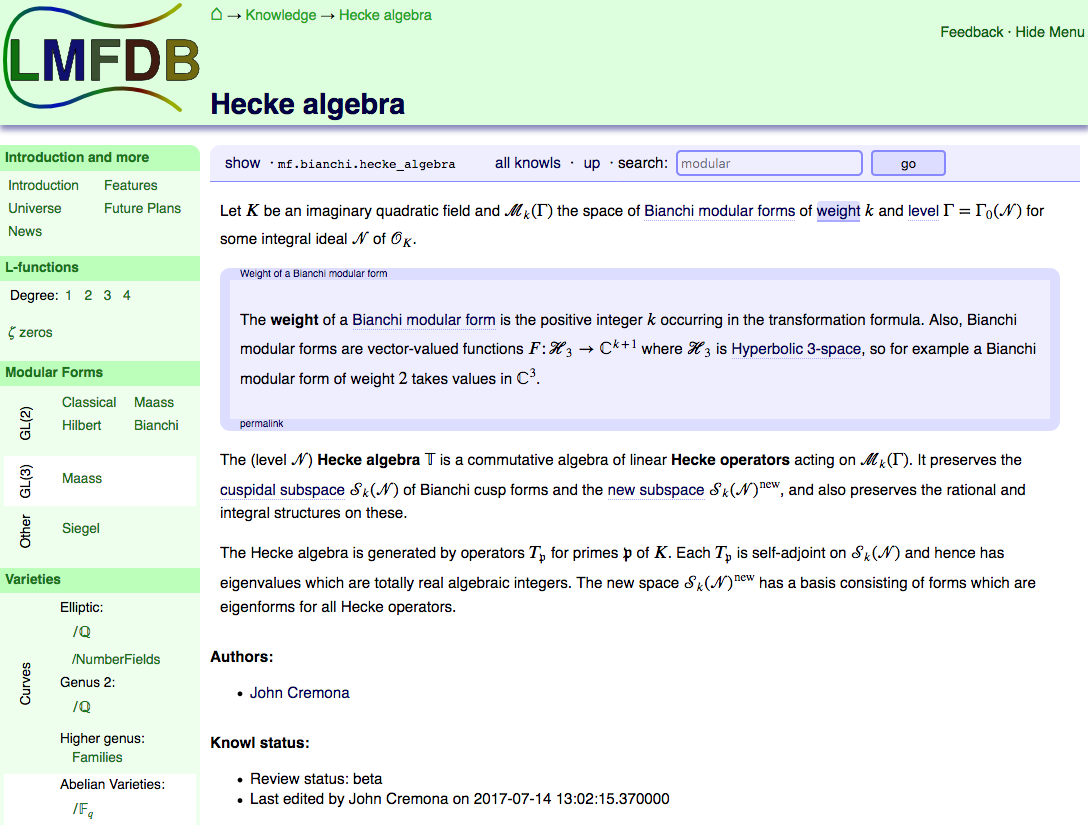
\includegraphics[width=14cm]{knowl}
  \caption{Knolws in the \LMFDB User Interface}\label{fig:knowl}
\end{figure}

\subsection{Alignments}\label{sec:integrating:alignments}

Finally we have to curate the \textbf{alignments} between the system dialects and the MitM ontology. 

To make the systems interoperable and translate objects and expressions, it is crucial to inform the system which symbols in the 
respective system API theories represent the same mathematical concepts. Then translation (as a first approximation) reduces to simply substituting symbols in an expression (see example below).\medskip

However, even when $A$ and $B$ deal with the ``same mathematical objects'', these may be constructed and represented differently, e.g., symbols can differ in name,
argument order/number, types, etc.
A major difficulty for system interoperability is correctly handling these subtle differences.
To formalize the details of this relation, \cite{MueGauKal:cacfms17} introduced \OMMT \textbf{alignments}.
Technically, these are pairs of \OMMT symbol identifiers decorated by a set of key-value pairs.
The alignments of $a$-symbols with the MitM ontology determine which $A$-objects correspond to MitM-objects.

The alignment of $a$-symbols to ontology symbols must be spelled out manually.
But this is usually straightforward and easy even for inexperienced users. For example, the following line aligns GAP's symbol \textsf{IsCyclic} (in the file \lstinline|lib/grp.gd|) with the corresponding symbol \textsf{cyclic} in the MitM ontology.
The key-value pairs are used to signify that this alignment is part of a group of alignments called ``VRE'' and can be used for translations in both directions.

\begin{lstlisting}
gap:/lib?grp?IsCyclic  mitm:/smglom/algebra?group?cylic
    direction="both" type="VRE"
\end{lstlisting}

Thus we can reduce the problem of interfacing $n$ systems to
\begin{inparaenum}[\em i\rm)]
\item curating the MitM ontology for the joint mathematical domain,
\item generating $n$ theory graphs for the system dialects,
\item maintaining $n$ collections of alignments with the MitM ontology.
\end{inparaenum}\medskip

For an example, consider again the dihedral group $D_4$ in \Sage (see Listings \ref{lst:sagedihedral:om} and \ref{lst:sagedihedral:xml}). We can align the relevant symbol 
\begin{lstlisting}
sage:?sage.groups.perm_gps.permgroup_named?DihedralGroup
\end{lstlisting}
with an abstract representation of dihedral groups in the MitM ontology (say, for instance \lstinline|mitm:?group?dihedralGroup|).
The \MMT system, when translating from \Sage to e.g. \GAP, then knows to replace the sage-specific symbol \lstinline|?DihedralGroup| by its system neutral equivalent in MitM, and the complex expression \lstinline+make_integer(4)+ by the plain OpenMath integer 4. To translate the resulting statement in MitM to \GAP, we only need to align \lstinline+mitm:?Groups?dihedralGroup+ with the constructor for dihedral groups in \GAP, namely \lstinline+gap:/grp?basic?DihedralGroupCons+. Translating to \GAP is then merely a matter of substituting this symbol in the OpenMath expression (\GAP already uses OpenMath integers for remote procedure calls via \SCSCP) to reconstruct the original \Sage object in \GAP. This yields the stepwise translation given in Figure \ref{fig:sagetogap}
\medskip

\begin{figure}\label{fig:sagetogap}

\begin{lstlisting}
sage:?sage.groups.perm_gps.permgroup_named?DihedralGroup
	mitm:?group?dihedralGroup 
	direction="both" type="VRE"
gap:/grp?basic?DihedralGroupCons							
	mitm:?group?dihedralGroup 
	direction="both" type="VRE"
\end{lstlisting}\medskip

\begin{tabular}{|lp{0.6\textwidth}|}\hline
\Sage & \lstinline|DihedralGroup(4)| \\
OpenMath (\Sage Dialect) & See Listing \ref{lst:sagedihedral:om} \\
OpenMath (MitM) & \lstinline|OMApplication(elem=OMSymbol(name='dihedralGroup', cd='group', cdbase='mitm'),arguments=[OMInteger(4)])| \\
OpenMath (\GAP Dialect) & \lstinline|OMApplication(elem=OMSymbol(name='DihedralGroupCons', cd='basic', cdbase='http://www.gap-system.org/grp'),arguments=[OMInteger(4)])| \\
	\GAP & \lstinline|DihedralGroupCons(4)|
\end{tabular}

\caption{Alignments and Stepwise Translation of Dihedral Group $D_4$ from \Sage to \GAP}
\end{figure}

Alignments form an independent part of the MitM interoperability infrastructure.
Incidentally, they obey a separate development schedule: the MitM ontology is developed by the community as a whole as the understanding of a mathematical domain changes.
The system dialects are released together with the systems according to their respective development cycle.
The alignments bridge between them and have to mediate these cycles.

These alignments are currently produced and curated using the approach, repository, and syntax described in~\cite{MueGauKal:cacfms17,MueRoYuRa:abtafs17}.
In the future, we will also consider automatically extracting alignments from the existing ad-hoc \Sage-to-$X$ translations.
These are (mainly) given as \Sage code annotations that relate \Sage operations and constructors with those of system $X$.

Figure~\ref{fig:cgtontology} shows some example alignments between symbols in the GAP content dictionary and the MitM ontology.




%%, but from some of the initial alignments and the \GAP API theories we will be able to infer more alignments automatically.
%%For example, the filter \texttt{GAP:IsGroup} is aligned with
%%\texttt{mitm:Group}, and the filter \texttt{GAP:IsPermGroup} is aligned with
%%\texttt{mitm:Subgroup SymmetricGroup [1..n]}.
%
%We formalized the theory of symmetric groups of a set in the MitM ontology.
%In \GAP, permutation groups are represented as subgroups (with finite support) of the symmetric group of $\mathbb{N}+$, and often one concretely has an isomorphism between the group one is interested in and a subgroup of $S_{\mathbb{N}+}$, for example via a group action.

%\texttt{SylowSubgroup}s are more difficult: They are special groups in their own right, namely groups whose size is a prime-power, but we also want them to be identified with a certain subgroup of the group we are working with.
%\ednote{MP: While I believe this to be an excellent additional example for \OMMT formalisation, this could be going too far for this paper}

%\ednote{MK@MK: still to write: the alignment-based priorization and suggestion mechanism. }


%%% Local Variables:
%%% mode: latex
%%% TeX-master: "report"
%%% End:

%  LocalWords:  DehKohKon:iop16 emph serialization sec:mitm deserializes subsubsection MueGauKal:cacfms17 MueRoYuRa:abtafs17 defemph defemph texttt texttt texttt texttt compactenum serializes lst:sagedihedral papertype ednote subtyping Cremona:LMFDB16,lmfdb:on knowls fig:knowl knowl knowl Kohlhase:ulsmf08 pdflatex flexiformal centering includegraphics Knolws inparaenum medskip MueGauKal:cacfms17,MueRoYuRa:abtafs17
%  LocalWords:  analyze itemize Deserialization serialized lstlisting pg_unreduce mathbb
%  LocalWords:  unpickle_global unreduce pg_DihedralGroup serializer py-openmath:on
%  LocalWords:  lstinline optimizations factorization serialize deserialized deserializer
%  LocalWords:  fig:cgtontology GroupHomset serializing analyzed py-scscp:on mitm:Group
%  LocalWords:  mitm:Subgroup SylowSubgroup newpart priorization summarize compactitem
%  LocalWords:  formalized

\section{\GAP/\Singular MitM Case Study}\label{sec:mitm_poc}
\subsection{MitM Protocol}\ednote{MK: Victor has connected \GAP and \Singular
  through standard OpenMath CDs and trivially aligning the systems, in
  particular the interface theory consists of an implementation of OpenMath CDs
  for polynomials and permutations}

For modular interaction between a Maths-in-the-Middle server, CAS \SCSCP servers 
and naive clients, we have developed the MitM/\SCSCP protocol that allows CAS 
servers to go online and offline independently of the MitM server. Below is the 
specification of the protocol.

\subsubsection{Peers}
One of the systems in the dialog must initially act as a server. This server will 
be called the MitM server and expose a strict set of function headers to clients 
upon startup. The other system will be referred to from now on as CAS (Computer 
Algebra System) and can expose an arbitrary set of function headers.

\subsubsection{Interaction}
The MitM server must, upon boot-up, expose the symbol "eq" from the CD 
"relation", as well as the following symbols from the CD "mitm\_transient"
over \SCSCP:
\begin{itemize}
  \item \textbf{registerServer}, taking one compulsory argument, the address of the
    CAS server as a string, and one optional argument, the port at which the CAS
    serves \SCSCP. If a port is not provided, it should default to 26133. This
    function should establish an \SCSCP connection with the CAS server at that 
    address and return the name/handler that the MitM server assigns to the 
    CAS instance as a string. This name is used when aligning functions.
  \item \textbf{registerFunction}, taking three arguments: the handler of the 
    server that exposes a symbol, the symbol that the server exposes, and
    a symbol in a global CD that it corresponds to. After this call, the MitM
    server should expose the global symbol as a function header and redirect
    calls to it to the CAS.
  \item \textbf{getAllServers}, taking no arguments. This function should return 
    the list of handlers for all the servers MitM is currently aware of.
  \item \textbf{removeFunction}, taking two arguments, the handler of a CAS server 
    and a symbol that that CAS exposes. After the call to this function no 
    requests should be redirected to that symbol on that CAS.
  \item \textbf{removeServer}, taking one argument- the name/handler that refers
    to the client connected to the CAS. This function should close the \SCSCP client
    to that CAS and stop serving functions that depend on symbols exposed by
    that CAS.
  \item \textbf{registerEquality}, taking three arguments: the handler of the 
    server that can compare applications of an OpenMath symbol, the function
    header exposed by that server that compares the applications, and the symbol
    that the server can compare. After this function call, any calls to the "eq"
    symbol with the applications of this symbol as arguments should be redirected
    to the CAS.
\end{itemize}

\subsection{Overview of the System}
In order to apply the MitM paradigm to practice, we have created a case study 
\cite{MitM-PoC} in which a user is able to access the functionality of two very 
different computer algebra systems by querying the MitM server that is 
implemented by an extension in MMT. The study consists of five components:
\begin{itemize}
  \item MitM server (as an MMT extension)
  \item \GAP \SCSCP server that specializes on computations in group theory
  \item \Singular \SCSCP server that specializes on polynomial calculations
  \item \Python client that uses the \SCSCP package
  \item \Python script that lines up the interactions between the MitM server and CAS servers
\end{itemize}

\begin{figure}[ht]\centering
  \begin{tikzpicture}[xscale=2, yscale=2]\normalsize
  \node[draw] (g) at (0,0) {
    \begin{tabular}{c}
      GAP Server \\GAP
    \end{tabular}
  };
  \node[draw] (m) at (2,0) {
    \begin{tabular}{c}
      MitM Server\\MMT
    \end{tabular}
  };
  \node[draw] (s) at (4,0) {
    \begin{tabular}{c}
      Singular Server\\Singuler(Python)
    \end{tabular}
  };
  \node[draw] (p) at (1, -1) {
    \begin{tabular}{c}
      Query Client\\Python
    \end{tabular}
  };
  \node[draw] (c) at (3, -1) {
    \begin{tabular}{c}
      Control Script\\Python
    \end{tabular}
    };
  \draw[->] (c) to node[right] {1} (m);
  \draw[->] (m) to[bend left=15] node[above] {2} (s);
  \draw[->] (m) to[bend right=15] node[above] {2} (g);
  \draw[->] (p) to node[left] {3} (m);
  \draw[->] (m) to[bend right=15] node[below] {4} (s);
  \draw[->] (m) to[bend left=15] node[below] {4} (g);
\end{tikzpicture}

%  LocalWords:  tikzpicture xscale yscale Singuler

  \caption[\GAP-\Singular MitM Interaction]{
    System Designed to Prove the Concept of the MitM Protocol
  }\label{fig:mitmpoc}
\end{figure}

The procedure illustrated in figure \ref{fig:mitmpoc} is as follows:
\begin{enumerate}
  \item The control script establishes an \SCSCP connection with the MMT MitM 
    server and aligns the functions exposed by the CAS (\GAP and \Singular) with
    global symbols.
  \item The MitM server establishes \SCSCP connections with the CAS server at
    provided addresses.
  \item The query client queries the MitM server for symbols from public CDs
    without any knowledge of the CAS in operation to calculate orbits of 
    polynomials.
  \item MitM server redirects the requests from the query client to the necessary
    CAS.
\end{enumerate}

\subsection{Components of the Study System}
\subsubsection{MMT MitM Server}
The MitM server is implemented as an MMT-shell extension. The integration into the
MMT ecosystem will be useful in the future for the automation of function 
alignment and type-checking of arguments. It is also queried via \SCSCP as opposed 
to QMT, because currently \SCSCP is more widely supported, e.g. by the \GAP and 
\Python packages.

\subsubsection{\GAP \SCSCP Server}
\GAP server uses the \GAP \SCSCP package to expose the minimal functions needed for 
this study- the constructor for a symmetric group of size N, and a function that
takes a list and a symmetric group and returns a permutation of the list for every 
member of the symmetric group that is obtained by applying that member to every
item of the list.

\subsubsection{\Singular \SCSCP Server}
Since \Singular currently doesn't have any support for \SCSCP, the \Singular \SCSCP server is
written in \Python using the \lstinline|scscp| and \lstinline|PySingular| python modules
and is adapted from the example code on the py-scscp repository\cite{PySCSCP}. The only
function exposed by this server is the evaluation of equality of two applications of the
DMP symbol.

\subsubsection{Controlling Client Script}
In the long term, the function alignment will be done automatically when a CAS 
informs the MitM server of its presence. Currently, however, the export of CAS 
type systems is still a work in progress, so the function alignment is done
via the MitM protocol. The job of the controlling script is thus to align the 
constructor of symmetric group of size N and the orbit of a list to their 
respective symbols in public CDs, as well as registering the ability of the 
\Singular server to equate polynomials.

\subsubsection{Naive Client}
The main client that queries the MitM server has no knowledge of the underlying 
CAS. It follows the procedure:
\begin{enumerate}
  \item Create an OpenMath polynomial.
  \item Obtain a symmetric group of size that is equal to the number of variables 
    in the polynomial from MitM.
  \item Using the obtained group, query MitM for all permutations of the list 
    of variables.
  \item Create polynomials from the permutations of the list of variables.
  \item Filter out the duplicate polynomials by querying MitM for equality of 
    polynomials.
\end{enumerate}
While this is very much a brute-force algorithm to calculate an orbit of a
polynomial, it showcases the ability of the client to query the MitM server that 
is then forced to use multiple CAS without the client needing any knowledge of the
underlying systems.

\subsection{Using the System}
\subsubsection{Dependencies}
The dependencies of the software in subject of the study and instructions on
acquiring them:
\begin{itemize}
  \item \textbf{Jupyter}- installed via pip
  \item \textbf{\GAP}- installed from https://github.com/gap-system/gap
  \item \textbf{\Singular}- installed via package manager or from
    https://www.singular.uni-kl.de/index.php/singular-download.html
  \item \textbf{MMT}- installed from https://github.com/Uniformal/MMT
  \item \textbf{Py-SCSCP}- installed via pip
  \item \textbf{PySingular}- installed via pip or from 
    https://github.com/sebasguts/SingularPython
\end{itemize}

\subsubsection{Execution}
Instructions on running the system:
\begin{itemize}
  \item Run singular\_server.py script using python, the gap\_server.g script
    using \GAP, and start MMT. From the MMT shell prompt, run 
    "file mitm\_server.msl".
  \item Run ControllingClient.py using python to set up alignments between
    MitM server and CAS servers.
  \item Start a Jupyter kernel using "jupyter notebook" and open the 
    QueryingClient.ipynb notebook. This is the example procedure that showcases
    a few examples of calculations of orbits of polynomials.
\end{itemize}

\subsection{Evaluation of the Study}
This study has implemented the MitM approach using \SCSCP, showing that the MitM 
paradigm is an achievable goal. Currently, however, the MitM server acts as 
merely a proxy, redirecting \SCSCP requests to CAS that know how to evaluate them.
For MitM to be a truly modular abstract algebra environment, the following
changes must be made:
\begin{itemize}
  \item A peer-to-peer connection must be made with the CAS servers, so that
    CAS servers can, in turn, query MitM if during a computation they encounter 
    a concept that lies outside their field of knowledge. In application to
    this particular case, it would be cleaner if, instead of asking MitM to 
    produce permutations of a list, the client simply queries MitM for the orbit 
    of a polynomial by defining an action of a member of the symmetric group on a 
    polynomial. \GAP would then be able to calculate the orbit by making the group 
    act on the polynomial with the described action and querying MitM for 
    equality of polynomials, resulting in a linear-time algorithm instead of
    quadratic-time behaviour displayed by the current client.
  \item Alignment between CAS servers and the MitM server must be automated.
    Although manual alignment as described in this case study is usable and
    enables pinpoint alignments to be made, it is not scalable. Any CAS that aims
    to be MitM-compatible should develop a representation of its type system
    in MMT, so that, upon establishing a connection with a new CAS system, the 
    MitM server would be able to automatically align newly accessible functions 
    with symbols from public CDs. This will also enable MMT to act as more than
    a routing proxy, as it would be able to typecheck the arguments of incoming
    requests, making the MitM system more rigid.
\end{itemize}

%%% Local Variables:
%%% mode: latex
%%% TeX-master: "paper"
%%% End:

%  LocalWords:  subsubsection mitm itemize textbf centering fig:mitmpoc lstinline scscp
%  LocalWords:  Jupyter _server.msl ControllingClient.py QueryingClient.ipynb bibitem
%  LocalWords:  thebibliography _server.msl sec:mitm_poc

\section{Conclusion}\label{sec:concl}

We have shown how to extend the Math-in-the-Middle framework for integrating systems to mathematical data bases like the \lmfdb. 
The main idea is to embed knowledge sources as virtual theories, i.e. theories that are not -- theoretically or in practice -- limited in the number of declarations and allow dynamic loading and processing. 
For accessing real-world knowledge sources, we have developed the notion of codecs and integrated them into the MitM ontology framework. 
These codec's (and their MitM types) lift knowledge source access to the MitM level and thus enable object-level interoperability and allow humans (mathematicians) access using the concepts they are familiar with. 
Finally, we have shown a prototypical query translation facility that allows to delegate some of the processing to the underlying knowledge source and thus avoid thrashing of virtual theories. 

\paragraph{Related Work} Most other integration schemes employ a \textbf{homogenous approach}, where there is a master sytsem and all data is converted into that system. 
A paradigmatic example of this is the Wolfram Language and the Wolfram Alpha search engine~\cite{WolframAlpha:on}, which are based on the Mathematica kernel. 
This is very flexible for anyone owning a Matheamtica license and experienced in the Mathematica language and environment.

The MitM-based approach to interoperability of data sources and systems proposed in this paper is inherently a \textbf{heterogeneous approach}: systems and data sources are kept ``as is'', but their APIs are documented in a machine-actionable way that can be utilized for remote procedure calls, content format mediation, and service discovery. 
As a consequence, interaction between systems is very flexible.
For the data source integration via virtual theories presented in this paper this is important. 
For instance, we can just make an extension of \mmt or Sage which just act as a programmatic interface for e.g. \lmfdb. 

\paragraph{Future Work}
We have discussed the MitM+virtual theories methodology on the elliptic curves sub-base of the \lmfdb, which we have fully integrated. 
We are currently working on additional \lmfdb sub-bases. 
The main problem to be solved is to elicit the information for the respective schema theories from the \lmfdb community. 
Once that is accomplished, specifying them in the format discussed in this paper and writing the respective codecs is straightforward. 

Moreover, we are working on integrating the the Online Encyclopedia of Integer Sequences (OEIS~\cite{Sloane:OEIS,oeis}). 
Here we have a different problem: the OEIS database is essentially a flat ASCII file with different slots (for initial segments of the sequences, references, comments, and formulae); all minimally marked up ASCII art. 
In~\cite{LuzKoh:fsarfo16} we have already (heuristically) flexiformalized OEIS contents in \ommt; the next step will be to come up with codecs based on this basis and develop schema theories for OEIS.

\subsubsection*{Acknowledgements}
The authors gratefully acknowledge the fruitful discussions with other participants of
work package WP6, in particular John Cremona on the LMFDB and Dennis M\"uller on early
versions of the \ommt-based integration. We acknowledge financial support from the
OpenDreamKit Horizon 2020 European Research Infrastructures project (\#676541).

%%% Local Variables:
%%% mode: latex
%%% TeX-master: "paper"
%%% End:

%  LocalWords:  sec:concl subsubsection ommt lmfdb itemize Sloane:OEIS,oeis LuzKoh:fsarfo16 flexiformalized MitM-based textbf utilized
  
  
\printbibliography
\end{document}
%%% Local Variables:
%%% mode: latex
%%% TeX-master: t
%%% End:

%  LocalWords:  maketitle twb sec:intro DehKohKon:iop16 MueGauKal:cacfms17 optimized mitm
%  LocalWords:  itemize MitM-based sec:concl twiesing:msc17 printbibliography sec:mitm
%  LocalWords:  sec:mmt summarize sec:cgt sec:ift MueRoYuRa:abtafs17,MueGauKal:cacfms17
%  LocalWords:  cgt concl apit newpage setcounter tocdepth tableofcontents mitm_poc
